\documentclass[a4j]{jarticle}
\usepackage[dvipdfmx]{graphicx}
\usepackage{here}
\usepackage{ascmac}
\usepackage{url}
\title{
\vspace{30mm}
株式会社マルナカ様\\
購入商品情報管理システム\\
外部設計書v1
\vspace{90mm}
}
\author{
株式会社Toron
}

\begin{document}
\maketitle
\newpage
\tableofcontents
\newpage

\section{ユーザインタフェース設計}

\subsection{画面詳細}

\subsubsection{購入履歴閲覧画面}

図\ref{welcome1}に管理者ページへのログインするためのページを示す。この画面では、ログインシステムの実装によって、管理者および各店舗の店長の判別を行うことができる。判別は、[ID]と[パスワード]によるベーシック認証によって行う。
\begin{figure}[H]
  \begin{center}
    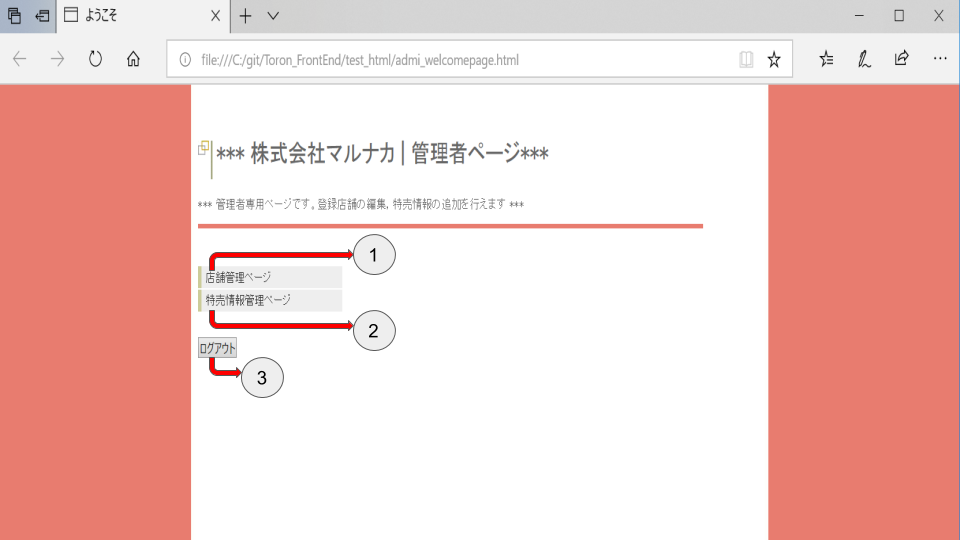
\includegraphics[width=15cm]{welcome1.png} \\
    \caption{ログイン画面}
    \label{welcome1}
  \end{cente
\end{figure}

\begin{enumerate}
	\item 管理者・店長ログインフォーム\\
	管理者および店長が所持しているIDとパスワードを入力するフォームである。
	\item 送信ボタン\\
	ログインフォームに入力されたIDとパスワードを用いて、データベースにあるユーザーテーブルと照合を行う。IDやパスワードが入力されていなかったり、整合されるアカウントがない場合には、ログインエラーとし、図\ref{login2}のような画面が表示される。IDとパスワードが認証され、そのユーザーが管理者である場合、後述する管理者ページへ遷移する。そのユーザーが店長である場合、後述する店長専用ページへ遷移する。
\end{enumerate}
\begin{figure}[H]
  \begin{center}
    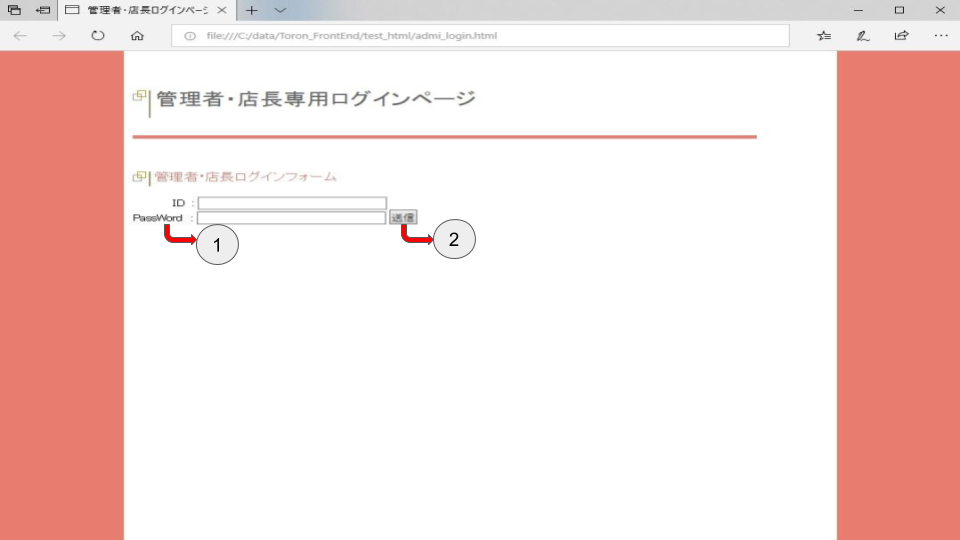
\includegraphics[width=15cm]{login.png} \\
    \caption{購入履歴閲覧画面}
    \label{login2}
  \end{center}
\end{figure}


\begin{enumerate}
\end{}
\end{document}
